
\begin{figure}[htb]
\pgfplotsset{
    width=12cm,
    tick label style={font=\footnotesize},
    label style={font=\small},
    legend style={font=\small},
}
\centering
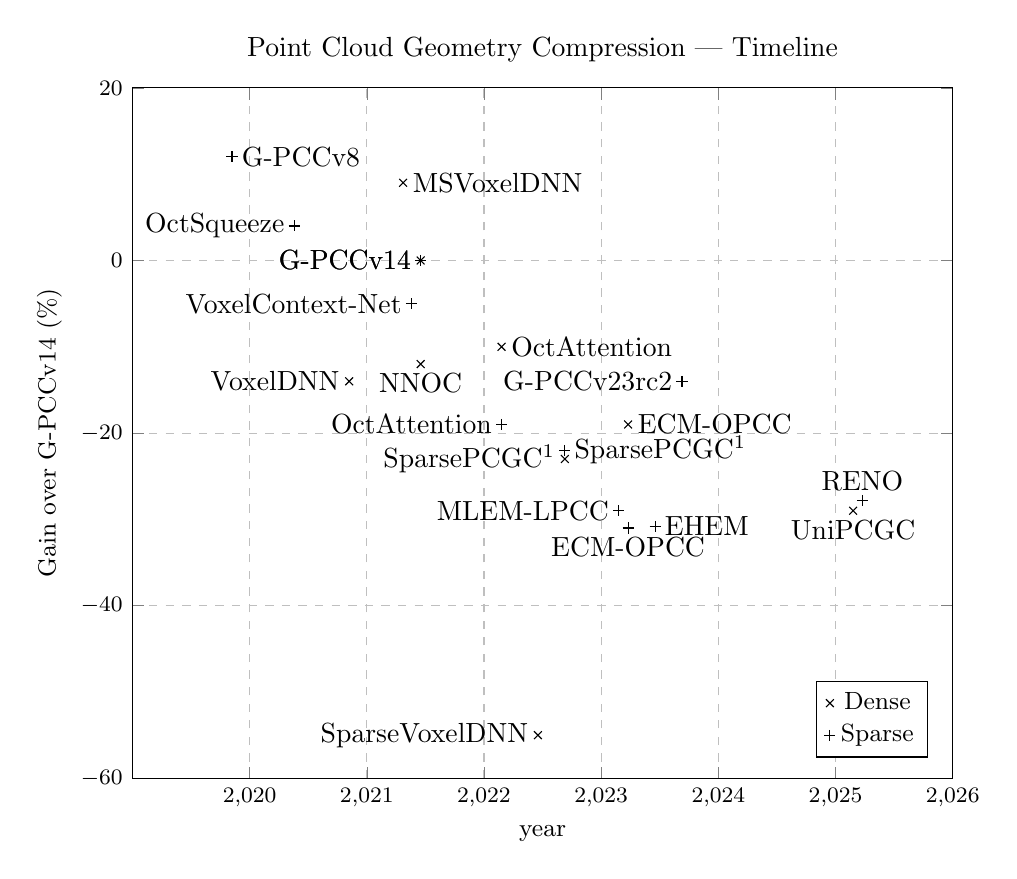
\begin{tikzpicture}
\begin{axis}[
    title={Point Cloud Geometry Compression --- Timeline},
    xlabel={year},
    ylabel={Gain over G-PCCv14 (\%)},
    xmin=2019, xmax=2026,
    ymin=-60, ymax=20,
    xtick={2020, 2021, 2022, 2023, 2024, 2025, 2026},
    ytick={-60, -40, -20, 0, 20},
    legend pos=south east,
    xmajorgrids=true,
    ymajorgrids=true,
    grid style=dashed,
]

\addplot[
    color=black,
    mark=x,
    only marks,
    point meta = explicit symbolic,
    nodes near coords,
    visualization depends on=\thisrow{align} \as \align,
    every node near coord/.style={anchor=\align}
]
table[meta=label] {
    x       y   label           align
    2020.85 -14  VoxelDNN        0
    2021.46 -12  NNOC            90
    2021.31 9    MSVoxelDNN      180
    2021.46 0    G-PCCv14        0
    2022.69 -23  SparsePCGC$^1$  0
    2022.15 -10  OctAttention    180
    2022.46 -55  SparseVoxelDNN  0
    2023.23 -19  ECM-OPCC        180
    2025.15 -29  UniPCGC         90
};
\addlegendentry{Dense}

\addplot[
    color=black,
    mark=+,
    only marks,
    point meta = explicit symbolic,
    nodes near coords,
    visualization depends on=\thisrow{align} \as \align,
    every node near coord/.style={anchor=\align}
]
table[meta=label] {
    x       y     label             align
    2019.85 12    G-PCCv8           180
    2020.38 4     OctSqueeze        0
    2021.38 -5    VoxelContext-Net  0
    2021.46 0     G-PCCv14          0
    2022.69 -22   SparsePCGC$^1$    180
    2022.15 -19   OctAttention      0
    2023.15 -29   MLEM-LPCC         0
    2023.23 -31   ECM-OPCC          90
    2023.46 -30.8 EHEM              180
    2023.69 -14   G-PCCv23rc2       0
    2025.23 -27.8 RENO              270
};
\addlegendentry{Sparse}
    
\end{axis}
\end{tikzpicture}
\caption{
The timeline of key publications in lossless point cloud geometric compression over the past half decade, illustrating the steady performance improvements achieved relative to the G-PCCv14 baseline.
$^1$SparsePCGC was originally published in November 2021 with comparatively lower performance due to hardware limitations at the time. With the advent of newer GPUs such as the NVIDIA RTX 4090, larger model configurations and reduced inference times have become feasible, resulting in significantly improved compression performance.
\label{fig:timeline}}
\end{figure}